\documentclass{beamer}

\usepackage{listings}
\usepackage{amsmath}
\usepackage[normalem]{ulem}
\usepackage{graphicx}

\frenchspacing

% Make Beamer less ugly:
\usefonttheme{serif}
\setbeamercolor{title}{fg=black}
\setbeamercolor{titlelike}{fg=black}
\setbeamercolor{frametitle}{fg=black}

\begin{document}

\title{MOS Technology 6502}
\subtitle{Architecture, Design, and Impact}
\author{Chris Ranc \\ Travis Whitaker}
\institute{Rochester Institute of Technolgoy}
\date{Spring 2016}
\maketitle

\begin{frame}
\frametitle{MOS Technology 6502 Overview}
\begin{columns}[T]
\begin{column}[T]{0.7\textwidth}
\begin{itemize}
\item Released in 1975 in 40-pin DIP package.
\item Competed directly with the Intel 8080 and Zilog Z80.
\item Lead to rapidly decreasing prices in the microprocessor market.
\item Widely popular in personal computer and system integration applications.
\item MOS acquired by Commodore in 1976.
\item Still used in embedded systems today.
\end{itemize}
\end{column}
\begin{column}[T]{0.3\textwidth}
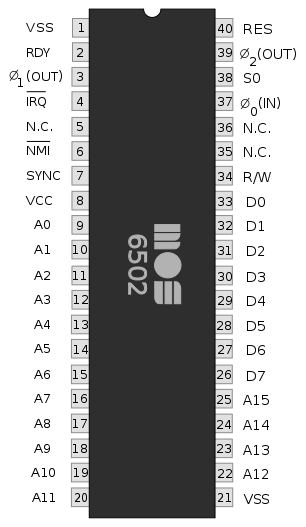
\includegraphics[scale=0.3]{images/MOS6502.png}
\end{column}
\end{columns}
\end{frame}

\begin{frame}
\frametitle{Specifications}
\begin{itemize}
\item 3 8-bit General Purpose Registers
\item 8-bit Stack Pointer
\item 8-bit Status Register
\item 16-bit Program Counter
\item 1 Edge-Triggered Non-Maskable Interrupt
\item 1 Maskable Level-Sensitive Interrupt
\item External Memory Address/Data Bus
\item RDY output for Hardware Step-Through
\end{itemize}
\end{frame}

\begin{frame}
\frametitle{History}
\begin{itemize}
\item Chuck Peddle noticed Motorola customers were frustrated with high 6800 unit cost.
\item Proposed a lower area, lower power, lower cost 6800 spin-off.
\item New design leverages depletion-mode metal oxide semiconductor transistors.
\item Frustrated by Motorola management, Peddle joins MOS Technology, who fund the 6502.
\item 1975 saw a recession impact the silicon industry; 6502 sales flop as a result.
\end{itemize}
\end{frame}

\begin{frame}
\frametitle{Beginnings of the Microcomputer}
\begin{columns}[T]
\begin{column}[T]{0.6\textwidth}
\begin{itemize}
\item To bolster sales, Peddle designs the MDT-650 single-board computer development platform.
\item MDT-650 extremely popular with both engineers and hobbyists.
\item Apple, Commodore, Atari, BBC capitalize on the emerging hobbyist/home computer market.
\item Apple II, Commodore PET \& VIC-20, BBC Micro, Atari 800 all designed around the 6502.
\end{itemize}
\end{column}
\begin{column}[T]{0.4\textwidth}
\begin{figure}
\centering
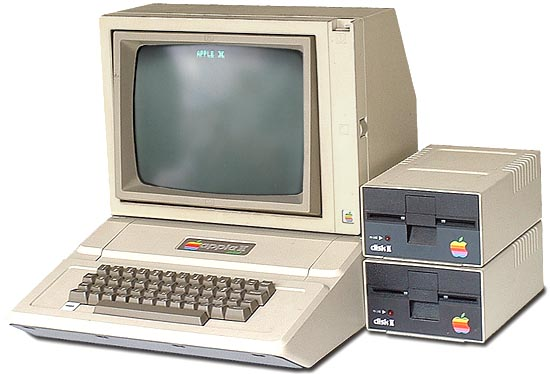
\includegraphics[scale=0.225]{images/appleii-system.jpg}
\end{figure}
\end{column}
\end{columns}
\end{frame}

\begin{frame}
\frametitle{Home Game Consoles Emerge}
\begin{itemize}
\item Ted Dabney and Nolan Bushnell begin investigating microprocessor-based video games.
\item Unlike previous games based on dedicated discrete logic, microprocessor-based systems could play multiple games.
\item Dabney and Bushnell realize that such a system would create it's own proprietary software market.
\item ``Stella'' prototype adapted to use the low-cost 6502 in 1975.
\item The Atari Video Computer System (later Atari 2600) was released in 1977.
\end{itemize}
\end{frame}

\begin{frame}
\frametitle{6502 in the Japanese Market}
\begin{itemize}
\item After success in the arcade game market, Nintendo decides to enter the personal computer market, work on the ``Advanced Video System'' begins.
\item Management decides that the keyboard and terminal will discourage non-technophiles from purchasing the system; controllers are the only remaining interface in the final design.
\item Engineers design a system around the cost-effective 6502, essentially unknown in Japan at the time.
\item Obscurity of the 6502 in the Japanese market led Nintendo to produce it's own proprietary cross-development platform.
\item The ``Famicom'' is released to critical acclaim in 1983.
\item The NES is released in the US in 1985.
\item Nintento's unified development platform and licensing model is still used in the console market today.
\end{itemize}
\end{frame}

\begin{frame}
\frametitle{6502 Implementation}
\begin{columns}[T]
\begin{column}[T]{0.5\textwidth}
\begin{figure}
\centering
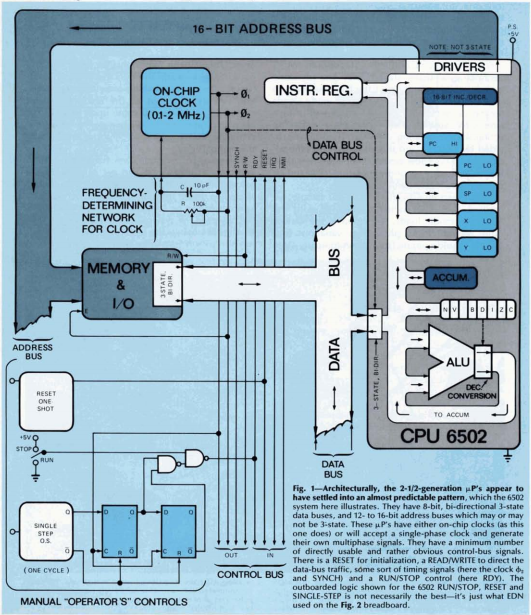
\includegraphics[scale=0.3]{images/cpu_layout.png}
\end{figure}
\end{column}
\begin{column}[T]{0.5\textwidth}
\begin{itemize}
\item 1-2 MHz typical clock frequency.
\item Two synchronizations per cycle.
\item Static PLA used for instruction decoding.
\item 2-stage concurrent fetch pipeline.
\item 3,510 total transistors.
\end{itemize}
\end{column}
\end{columns}
\end{frame}

\begin{frame}
\frametitle{6502 Polysilicon Diffusion Layers}
\begin{figure}
\centering
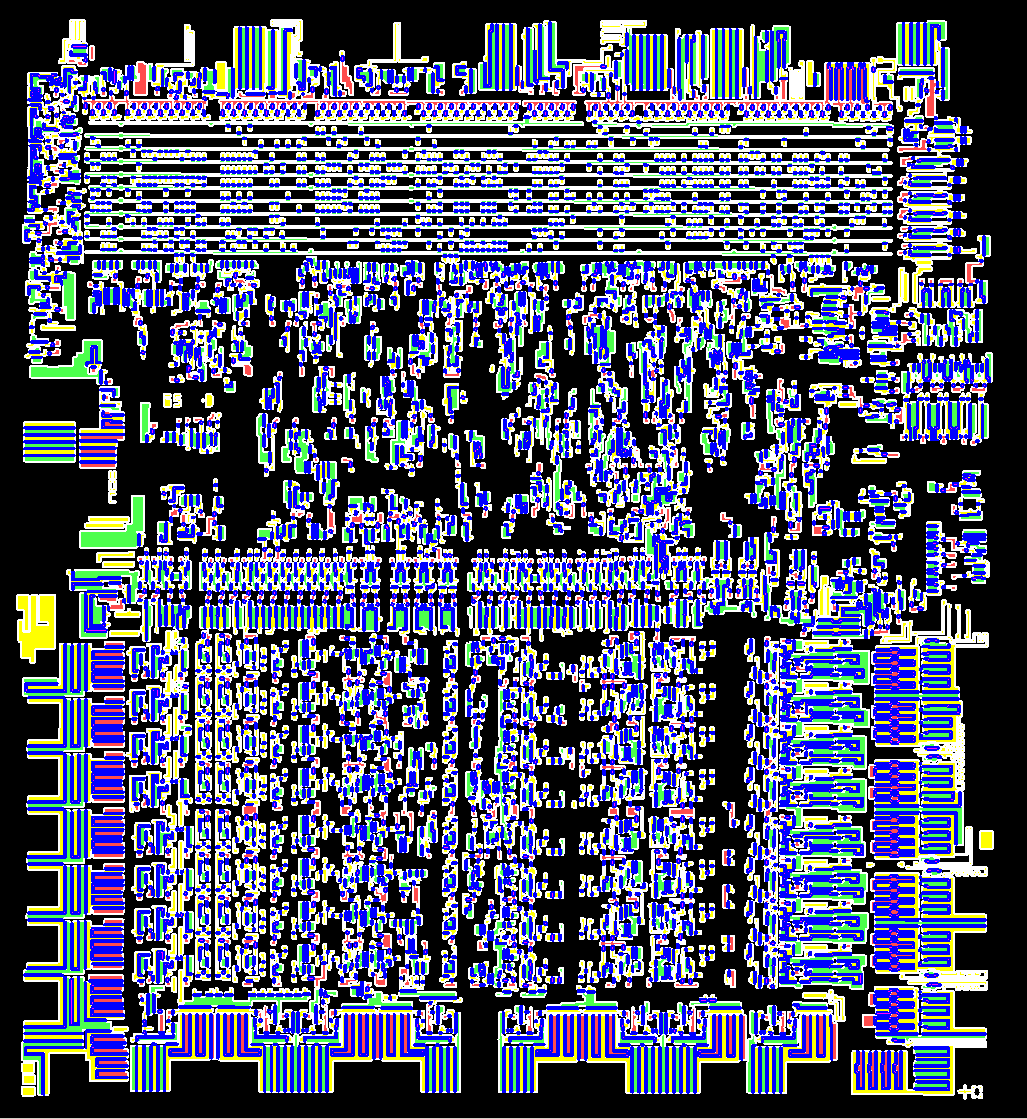
\includegraphics[scale=0.2]{images/polylayers.png}
\end{figure}
\end{frame}

\begin{frame}
\frametitle{6502 Layer Overlay}
\begin{figure}
\centering
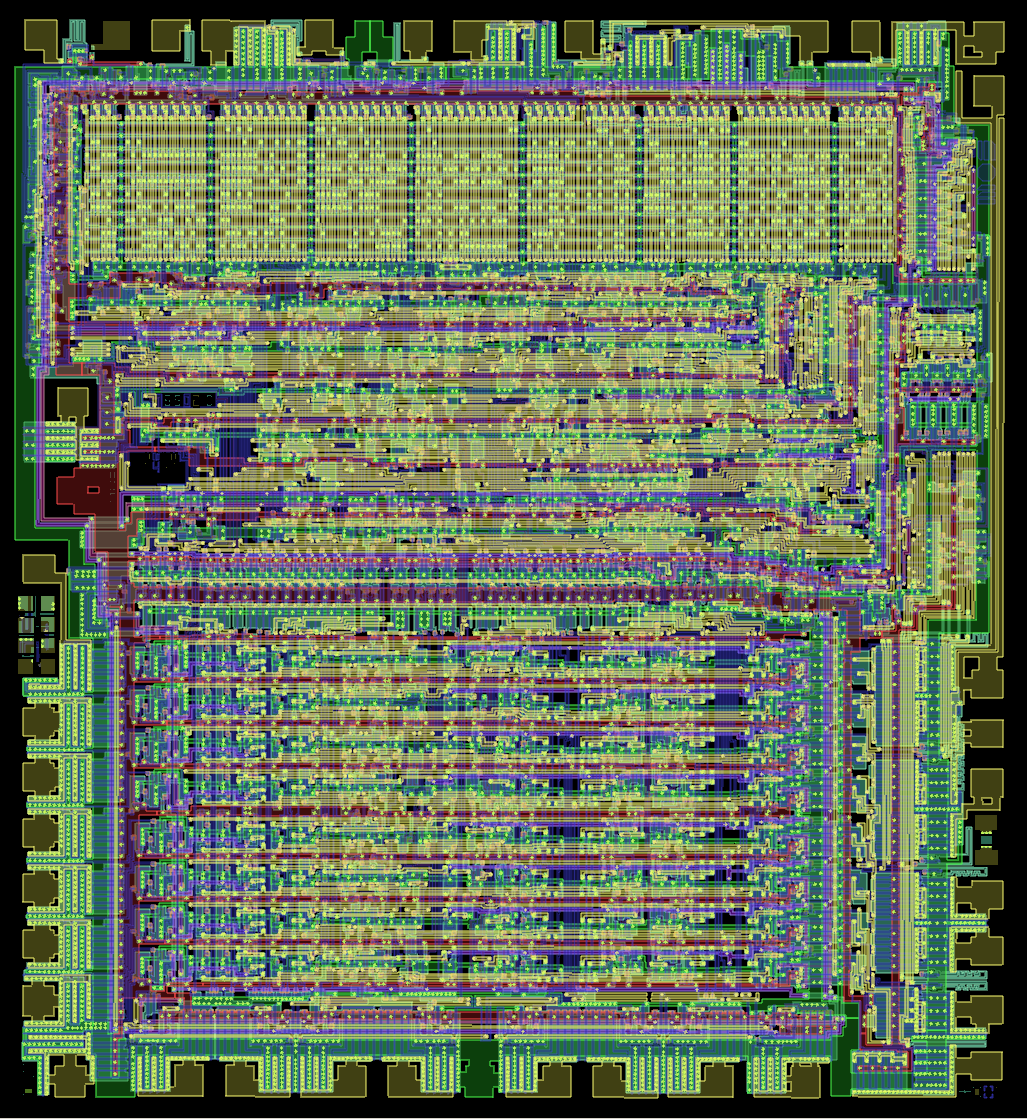
\includegraphics[scale=0.17]{images/all.png}
\item {6502 Visualization: \url http://www.visual6502.org/JSSim/index.html}
\end{figure}
\end{frame}

\begin{frame}
\frametitle{Addressing Modes}
\begin{columns}[T]
\begin{column}[T]{0.5\textwidth}
\begin{itemize}
\item Absolute (Immediate Address)
\item Branch-relative
\item Zero Page
\item Absolute/Zero-Page Indirection
\end{itemize}
\end{column}
\begin{column}[T]{0.5\textwidth}
\begin{figure}
\centering
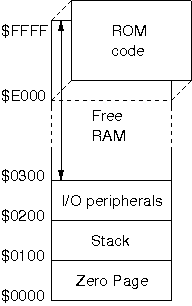
\includegraphics[scale=0.6]{images/mmap.png}
\end{figure}
\end{column}
\end{columns}
\end{frame}

\end{document}
